\documentclass[conference]{IEEEtran}
\IEEEoverridecommandlockouts

\usepackage[utf8]{inputenc}
\usepackage{cite}
\usepackage{amsmath,amssymb,amsfonts}
\usepackage{booktabs}
\usepackage{array}
\usepackage{graphicx}
\usepackage{textcomp}
\usepackage{xcolor}
\usepackage{url}
\usepackage[hidelinks]{hyperref}

\def\BibTeX{{\rm B\kern-.05em{\sc i\kern-.025em b}\kern-.08em
    T\kern-.1667em\lower.7ex\hbox{E}\kern-.125emX}}

\hypersetup{
  pdftitle={Transformer-Based Semantic Mapping of Cyber Threat Intelligence to MITRE ATT\&CK Techniques: A Retrieval and Reranking Benchmark},
  pdfauthor={Douglas Felipe de Lima Silva},
  pdfsubject={Cyber threat intelligence, MITRE ATT\&CK, semantic retrieval, cross-encoder reranking},
  pdfkeywords={cyber threat intelligence; MITRE ATT\&CK; information retrieval; sentence transformers; reranking}
}

\begin{document}

\title{Transformer-Based Semantic Mapping of Cyber Threat Intelligence to MITRE ATT\&CK Techniques: A Retrieval and Reranking Benchmark}

\author{
\IEEEauthorblockN{Douglas Felipe de Lima Silva}
\IEEEauthorblockA{
\textit{Instituto Metrópole Digital} \\
\textit{Universidade Federal do Rio Grande do Norte} \\
Natal, Brazil \\
pesquisadoug@gmail.com \\
ORCID: \href{https://orcid.org/0009-0007-9868-4891}{0009-0007-9868-4891}
}
}

\maketitle

\begin{abstract}
Mapping unstructured cyber threat intelligence (CTI) procedure descriptions to MITRE ATT\&CK techniques is a recurring requirement for threat analysis, reporting, and security operations. This paper presents a reproducible benchmark for zero-shot semantic mapping of ATT\&CK-derived procedure descriptions to Enterprise ATT\&CK techniques and sub-techniques. The benchmark was built from the official Enterprise ATT\&CK STIX 2.1 bundle and contains 697 active candidate techniques, 17,030 procedure-query instances, and a stricter subset of 14,868 queries after exact target ATT\&CK identifiers and exact target technique names were removed. Four retrieval settings were evaluated: TF-IDF, BM25, a MiniLM sentence-transformer bi-encoder, and MiniLM bi-encoder retrieval followed by cross-encoder reranking of the top-20 candidates. In the strict subset, the bi-encoder improved nDCG@10 from 0.3775 for TF-IDF and 0.3411 for BM25 to 0.4478. Cross-encoder reranking further increased nDCG@10 to 0.4915 and MRR@10 to 0.4310, at the cost of substantially higher query latency. The results indicate that pretrained Transformer retrieval models improve ATT\&CK technique ranking under the evaluated conditions, while also exposing a quality-latency trade-off that must be considered before operational deployment.
\end{abstract}

\begin{IEEEkeywords}
cyber threat intelligence, MITRE ATT\&CK, semantic search, information retrieval, sentence transformers, cross-encoder reranking
\end{IEEEkeywords}

\section{Introduction}
Cyber threat intelligence reports often describe adversary behavior as free text, whereas defensive analytics, detection engineering, and incident reporting commonly require normalized references to MITRE ATT\&CK techniques. This normalization step is labor-intensive because procedure descriptions can mention tools, campaigns, threat groups, infrastructure, or behavior without explicitly naming the target technique. The resulting mapping problem is naturally framed as information retrieval: given a CTI procedure description, rank the ATT\&CK techniques most likely to represent the described behavior.

MITRE ATT\&CK provides a public knowledge base of adversary tactics and techniques based on observed behavior \cite{mitre_attack}. Its STIX representation enables reproducible extraction of techniques, relationships, and procedure examples \cite{mitre_attack_stix_data}. Framing ATT\&CK mapping as information retrieval---ranking candidate techniques for a given procedure description---makes it possible to reuse standard IR evaluation methodology (ranking cutoffs, recall, reciprocal rank, nDCG) and to compare lexical and neural retrieval methods under the same protocol.

A benchmark derived from ATT\&CK itself, however, must account for leakage. Some procedure descriptions contain the exact ATT\&CK identifier or the exact technique name, which can inflate lexical matching results and obscure the value of semantic retrieval: a query that already contains the string ``T1566'' or ``Phishing'' makes the mapping problem far easier than the general case that a human analyst faces when reading a report that does not name the technique explicitly. This motivates comparing lexical retrieval (TF-IDF, BM25), dense semantic retrieval (a sentence-transformer bi-encoder), and cross-encoder reranking, and reporting results both on the full query set and on a stricter subset from which exact target-identifier and exact target-name occurrences have been removed.

The main contributions of this work are:
\begin{itemize}
\item a reproducible benchmark and experimental pipeline that constructs a candidate corpus from active Enterprise ATT\&CK techniques and sub-techniques directly from the official STIX 2.1 bundle;
\item construction of multi-relevance procedure queries from active STIX \texttt{uses} relationships, with an explicit, auditable leakage-detection rule for exact target identifiers and exact target names;
\item an evaluation protocol that reports both all-query and strict-query (leakage-audited) results under the same top-10 ranking metrics, enabling a comparison of TF-IDF, BM25, a MiniLM bi-encoder, and MiniLM bi-encoder retrieval followed by cross-encoder reranking;
\item statistical uncertainty estimates (bootstrap confidence intervals) for the main ranking-quality claims, together with computational-efficiency measurements and an exploratory attention/error analysis, released with full reproducibility artifacts (manifest, per-query metrics, model metadata, software/environment versions).
\end{itemize}
This study does not claim novelty in the underlying retrieval or reranking algorithms, which are established components; the contribution is the leakage-aware, reproducible benchmark construction and evaluation protocol applied to ATT\&CK-derived CTI mapping.

\section{Background and Related Work}
\subsection{MITRE ATT\&CK and CTI Normalization}
ATT\&CK is widely used as a shared vocabulary for adversary tactics, techniques, and procedures. In machine-readable form, the ATT\&CK STIX data expose attack-pattern objects, software and group objects, and relationships among them. This makes it possible to construct a retrieval task in which technique descriptions are candidate documents and procedure descriptions are queries. Surveys of ATT\&CK usage in research and practice report that the framework is applied across threat modeling, detection engineering, and CTI structuring, and identify automatic technique mapping from unstructured text as an active and only partially solved problem \cite{roy2023sok}.

\subsection{TTP Extraction and ATT\&CK Technique Mapping from CTI Text}
A substantial line of work extracts tactics, techniques, and procedures (TTPs) from unstructured CTI text. Husari et al. proposed TTPDrill, which combines information extraction and threat-ontology matching to translate free-text CTI reports into structured threat actions and kill-chain phases \cite{husari2017ttpdrill}. Legoy et al. framed ATT\&CK tactic and technique labeling as a multi-label text classification problem and released rcATT, a classifier-based tool trained on ATT\&CK procedure text \cite{legoy2020automated}. Orbinato et al. conducted an experimental study comparing traditional and Transformer-based machine-learning classifiers, including BERT, for mapping unstructured CTI sentences to ATT\&CK techniques, and analyzed the main sources of classification error \cite{orbinato2022automatic}.

These studies predominantly formulate ATT\&CK mapping as \emph{supervised multi-class or multi-label classification} over a fixed technique taxonomy, trained and evaluated on curated or crowd-labeled CTI report corpora external to ATT\&CK itself. In contrast, the present benchmark formulates the task as \emph{zero-shot ranking/retrieval} over the technique catalog, without any ATT\&CK-specific supervised fine-tuning, and constructs both queries and candidates directly and reproducibly from the official ATT\&CK STIX bundle rather than from a separately curated report corpus. This retrieval formulation naturally returns a ranked list of candidate techniques (useful when more than one technique is plausible) rather than a single predicted label, and it lets the same evaluation protocol compare lexical and neural methods without retraining a classifier per method.

\subsection{Lexical and Neural Retrieval}
Classical information retrieval methods such as TF-IDF cosine similarity and BM25 remain strong baselines for sparse lexical matching \cite{manning2008introduction,robertson2009probabilistic}. This benchmark uses the \texttt{rank\_bm25} implementation of BM25Okapi \cite{rankbm25}. The effectiveness of these lexical methods depends on token overlap between the query and candidate text. Neural sentence encoders, including Sentence-BERT style bi-encoders \cite{reimers2019sentencebert}, instead embed text into a dense vector space and can retrieve semantically related candidates even when exact wording differs. MiniLM compresses Transformer representations for lower-cost inference \cite{wang2020minilm}, making it suitable for lightweight retrieval experiments.

\subsection{Reranking}
Bi-encoders are efficient because queries and candidates can be embedded separately. Cross-encoders score query-candidate pairs jointly, which is typically more expensive but can improve ranking quality. The cross-encoder used in this study was pretrained on MS MARCO style passage-ranking data \cite{bajaj2016msmarco}. In this benchmark it is used only for reranking the bi-encoder top-20 candidates, so it cannot recover relevant techniques absent from that candidate set.

\subsection{Positioning of This Benchmark}
Relative to prior TTP-extraction and ATT\&CK-classification work, this benchmark differs in three respects. First, it evaluates \emph{retrieval and reranking} rather than classification, comparing lexical, dense bi-encoder, and cross-encoder methods under one shared ranking protocol and metric set. Second, queries and candidate documents are both constructed programmatically from the official ATT\&CK STIX bundle, which keeps corpus construction fully reproducible but also means the benchmark evaluates ATT\&CK-derived semantic mapping rather than mapping from independently collected, real-world CTI reports (see Limitations). Third, it introduces an explicit, auditable leakage rule that separates an \emph{all-query} evaluation from a \emph{strict-query} evaluation with exact target-identifier and exact target-name occurrences removed; among the retrieval-based ATT\&CK-mapping studies reviewed for this work, this all/strict leakage split does not appear to be standard practice, and it is intended to make explicit how much of a lexical method's apparent performance is attributable to trivial string overlap with the target label rather than semantic correspondence.

Recent work has begun to apply large language models directly to ATT\&CK-oriented CTI tasks. B\"uchel et al. present a systematization of automated TTP extraction from CTI reports, highlighting persistent gaps between reported and practically achievable extraction quality across existing tools and datasets \cite{buchel2025sok}. Lekssays et al. propose TechniqueRAG, a retrieval-augmented generation framework that couples off-the-shelf retrievers with instruction-tuned LLMs and zero-shot reranking for adversarial technique annotation \cite{lekssays2025techniquerag}, which is closely related in spirit to the retrieval-plus-reranking pipeline evaluated here but targets free-form CTI narratives with an LLM-based reranker rather than an ATT\&CK-derived benchmark with a cross-encoder. Cheng et al. introduce CTIConnect, a benchmark for retrieval-augmented LLMs spanning multiple heterogeneous CTI sources, including CVE, CWE, CAPEC, and ATT\&CK \cite{cheng2025cticonnect}. These studies motivate the present benchmark's narrower, leakage-audited focus on ATT\&CK-derived retrieval and reranking as a controlled complement to broader LLM-based CTI evaluations.

\section{Materials and Methods}
\subsection{Data Source}
The benchmark was constructed from the official Enterprise ATT\&CK STIX 2.1 bundle. The executed manifest records the source URL, SHA-256 hash, STIX object count, and latest object modification timestamp. The evaluated bundle contained 26,086 STIX objects and the latest object modification timestamp was 2026-08-05T21:33:58.496Z.

\subsection{Candidate Corpus}
Candidate documents were active Enterprise ATT\&CK \texttt{attack-pattern} objects corresponding to techniques and sub-techniques. Revoked and deprecated objects were excluded. Each candidate document concatenated the ATT\&CK identifier, technique name, and technique description. The full run produced 697 candidate techniques and sub-techniques.

\subsection{Procedure Queries and Relevance Labels}
Queries were extracted from active STIX \texttt{relationship} objects whose \texttt{relationship\_type} was \texttt{uses}, whose source object was active, whose target object was an eligible candidate technique, and whose relationship description was non-empty. Query text concatenated the source object name and cleaned procedure description. To preserve multi-relevance, procedure examples were grouped by source object reference and normalized description; a single query could therefore have more than one relevant ATT\&CK technique. Queries shorter than 20 characters after cleaning were discarded. The full benchmark contained 17,030 evaluation queries, including 91 multi-relevant queries.

\subsection{Text Preprocessing}
Three preprocessing operations were implemented and are used consistently for technique documents and query text. (1) \emph{Cleaning} (\texttt{clean\_attack\_text}): HTML entities are unescaped, Markdown-style links \texttt{[text](url)} are collapsed to their link text, ATT\&CK-style \texttt{(Citation: ...)} references are removed, remaining HTML tags are stripped, non-breaking spaces are replaced with ordinary spaces, and consecutive whitespace is collapsed to a single space with leading/trailing whitespace trimmed. No stemming, stop-word removal, or lowercasing is applied at this stage, so candidate and query text retain original casing and punctuation. (2) \emph{Audit normalization} (\texttt{normalize\_for\_audit}), used only for leakage detection: cleaned text is lowercased and every character other than \texttt{[a-z0-9.]} is replaced with a space, followed by whitespace collapsing. (3) \emph{Lexical tokenization} (\texttt{simple\_tokenize}), used only for BM25 indexing and querying: cleaned text is lowercased and tokenized with the regular expression \texttt{[a-z0-9][a-z0-9./\_-]*}, i.e., alphanumeric tokens that may internally contain periods, underscores, hyphens, or slashes (so that identifiers such as \texttt{T1566.001} or \texttt{rundll32.exe} remain single tokens). Candidate documents concatenate the ATT\&CK identifier, technique name, and description (\texttt{"<ID>. <name>. <description>"}); queries concatenate the source object name and procedure description. Duplicate technique identifiers are removed by keeping the first occurrence per \texttt{attack\_id}; duplicate queries are avoided by construction because procedure examples are grouped by source reference and normalized description before query text is generated.

\subsection{Leakage Audit}
Two evaluation subsets were reported. The \emph{all} subset used all 17,030 queries. The \emph{strict} subset was constructed by excluding queries containing an exact relevant ATT\&CK identifier or exact relevant technique name in the audit-normalized query text (case-insensitive; technique names shorter than 4 normalized characters were not used as leakage triggers, to avoid spurious matches on very short names). The audit found zero exact target-identifier leakage queries and 2,162 exact target-name leakage queries, leaving 14,868 strict queries (87.30\% of the all-query set). This rule excludes queries containing explicit target-identifier and target-name matches but does not guarantee the absence of all lexical overlap (e.g., partial name overlap or shared vocabulary between the query and the correct technique description can still occur).

\subsection{TF-IDF Configuration}
TF-IDF used scikit-learn's \texttt{TfidfVectorizer} with \texttt{lowercase=True}, word \texttt{ngram\_range=(1,2)} (unigrams and bigrams), \texttt{min\_df=1}, \texttt{sublinear\_tf=True}, and \texttt{max\_features=50000}. All other parameters used scikit-learn defaults, including the default English tokenizer/analyzer (token pattern \texttt{(?u)\textbackslash b\textbackslash w\textbackslash w+\textbackslash b}), \texttt{max\_df=1.0}, no stop-word removal, L2 row normalization, and \texttt{smooth\_idf=True}. Query-candidate similarity was cosine similarity between the TF-IDF vectors of the query and every candidate document.

\subsection{BM25 Configuration}
BM25 used the \texttt{rank\_bm25} package's \texttt{BM25Okapi} implementation \cite{rankbm25} with its default parameters ($k_1=1.5$, $b=0.75$, no non-default arguments). Candidate and query text were tokenized with the custom \texttt{simple\_tokenize} regular-expression tokenizer described above (lowercase alphanumeric tokens, no stemming or stop-word removal); \texttt{rank\_bm25} itself performs no text preprocessing, so tokenization was applied identically to the candidate corpus and to each query before indexing/scoring.

\subsection{Bi-Encoder Configuration}
The dense bi-encoder was \texttt{sentence-transformers/all-MiniLM-L6-v2}, loaded via the \texttt{sentence-transformers} library at Hugging Face commit \texttt{1110a243} (abbreviated; the full 40-character hash is recorded in \texttt{results/model\_metadata.json}). The model produces 384-dimensional embeddings (mean pooling, as defined by the model's default pooling configuration); embeddings for both candidate techniques and queries were L2-normalized (\texttt{normalize\_embeddings=True}), so that the dot product used for ranking is equivalent to cosine similarity. Candidate technique embeddings were precomputed once and cached; batch size was 32 on the CPU execution reported here (the pipeline uses batch size 128 automatically if a CUDA device is available, but the reported run used \texttt{torch\_device=cpu}). The model has 22{,}713{,}216 parameters (86.64 MiB in float32). No maximum-sequence-length override was applied beyond the model's default tokenizer truncation behavior.

\subsection{Cross-Encoder Reranking Configuration}
Reranking used \url{cross-encoder/ms-marco-MiniLM-L6-v2} (Hugging Face commit \texttt{233902d2}, abbreviated; full hash in \texttt{results/model\_metadata.json}), applied only to the bi-encoder's top-20 candidates per query (\texttt{rerank\_top\_k=20}). For each query, 20 (query, candidate-document) text pairs were constructed and scored jointly by the cross-encoder; candidates were then re-sorted in descending order of the cross-encoder score, replacing the bi-encoder order within that top-20 set. Batch size was 16 on CPU (64 on CUDA, unused in the reported run). Because reranking operates strictly within the bi-encoder top-20, it \emph{cannot recover} a relevant technique that the bi-encoder failed to place in its top-20 candidates for that query; this is an explicit and preserved limitation of the reranking stage (Section~\ref{sec:limitations}).

\subsection{Metrics}
The ranking cutoff for reporting was 10. The benchmark reports Recall@1, Recall@5, Recall@10, Hit@1, Hit@5, Hit@10, MRR@10, nDCG@10, and MAP@10; all nine metrics are computed by the pipeline for every method/subset combination and are available in \texttt{results/metrics.csv} and \texttt{results/per\_query\_metrics.csv}. For table width, this manuscript's main results table (Table~\ref{tab:metrics}) reports Recall@1, Recall@5, Recall@10, MRR@10, nDCG@10, and MAP@10; the complete metric set, including all Hit@k values, is provided in the repository's reproducibility artifacts. Binary relevance was used throughout: a candidate technique is relevant to a query if its ATT\&CK identifier is a member of that query's relevant-technique set (which may contain more than one identifier for the 91 multi-relevant queries). Recall@k is the fraction of a query's relevant techniques retrieved in the top-$k$ list; Hit@k is 1 if at least one relevant technique is retrieved in the top-$k$ list and 0 otherwise; MRR@10 is the reciprocal rank of the first relevant technique within the top 10 (0 if none is found); nDCG@10 and MAP@10 use binary relevance gains within the top-10 cutoff, with the ideal ranking for nDCG@10 capped at $\min(|\text{relevant}|, 10)$.

\subsection{Statistical Uncertainty}
\label{sec:bootstrap}
To quantify sampling uncertainty over queries, 95\% confidence intervals were computed with the non-parametric bootstrap over queries, using 10{,}000 resamples with replacement and a fixed random seed (42), implemented with NumPy's \texttt{Generator.integers} for resampling and the 2.5th/97.5th percentiles of the bootstrap distribution as interval bounds. Single-method intervals resample per-query metric values independently. Improvement intervals (bi-encoder vs. TF-IDF/BM25, and bi-encoder+cross-encoder vs. bi-encoder) resample the same bootstrap query indices for both methods being compared (paired resampling by \texttt{query\_id}), so that each bootstrap replicate reflects the same random subset of queries for both methods. All confidence intervals reported in Section~\ref{sec:results} were computed from \texttt{results/per\_query\_metrics.csv} and are also saved to \texttt{results/bootstrap\_ci.json} for independent verification.

\subsection{Efficiency and Reproducibility}
Efficiency measurements included indexing time, mean query latency, parameter count, parameter-memory footprint, and local artifact size where applicable. The full experiment was executed on CPU with Python 3.12.0, PyTorch 2.14.0+cpu, Transformers 5.17.0, Sentence-Transformers 6.0.1, NumPy 2.5.3, pandas 3.0.5, SciPy 1.18.1, and scikit-learn 1.9.1, on a Windows 11 workstation with an Intel Core i7-14700K CPU (20 physical cores, 28 logical threads) and 32~GiB RAM. Latency figures are CPU wall-clock means over the full query set (17,030 queries; no separate warm-up phase or repeated timed trials were used, so reported latency reflects a single full pass rather than an average of multiple repetitions). Bi-encoder query latency includes query tokenization and encoding plus similarity scoring against precomputed, cached candidate embeddings; TF-IDF and BM25 latency include query vectorization/tokenization and scoring; cross-encoder latency is the mean per-query pair-scoring time added on top of the bi-encoder retrieval that produces its top-20 input candidates. Disk I/O for model loading is excluded from the reported per-query latency. The full pipeline generated manifests, metrics, per-query metrics, rankings, efficiency summaries, model metadata, attention inspection outputs, and paper figures.

\section{Results}
\label{sec:results}
\subsection{Benchmark Characteristics}
Table~\ref{tab:dataset} summarizes the benchmark produced by the full execution. The strict subset retained 87.30\% of the all-query set after exact target-name leakage removal.

\begin{table}[htbp]
\caption{Full Benchmark Characteristics}
\label{tab:dataset}
\centering
\begin{tabular}{lr}
\toprule
\textbf{Property} & \textbf{Value} \\
\midrule
STIX objects & 26,086 \\
Candidate techniques/sub-techniques & 697 \\
All procedure queries & 17,030 \\
Strict procedure queries & 14,868 \\
Exact target-ID leakage queries & 0 \\
Exact target-name leakage queries & 2,162 \\
Multi-relevant queries & 91 \\
Rerank candidate depth & 20 \\
\bottomrule
\end{tabular}
\end{table}

\subsection{Retrieval Quality}
Table~\ref{tab:metrics} reports the main top-10 metrics for the all and strict subsets. In both subsets, the MiniLM bi-encoder outperformed lexical baselines. On the strict subset, the bi-encoder achieved Recall@10 of 0.6467, MRR@10 of 0.3862, and nDCG@10 of 0.4478. Cross-encoder reranking further improved strict Recall@10 to 0.6853, MRR@10 to 0.4310, and nDCG@10 to 0.4915.

\begin{table*}[htbp]
\caption{Retrieval and Reranking Results on Full Evaluation}
\label{tab:metrics}
\centering
\scriptsize
\begin{tabular}{llrrrrrr}
\toprule
\textbf{Subset} & \textbf{Method} & \textbf{Recall@1} & \textbf{Recall@5} & \textbf{Recall@10} & \textbf{MRR@10} & \textbf{nDCG@10} & \textbf{MAP@10} \\
\midrule
All & TF-IDF & 0.2715 & 0.4919 & 0.5945 & 0.3667 & 0.4204 & 0.3660 \\
All & BM25 & 0.2382 & 0.4444 & 0.5293 & 0.3263 & 0.3744 & 0.3258 \\
All & MiniLM-BiEncoder & 0.3004 & 0.5615 & 0.6709 & 0.4128 & 0.4740 & 0.4120 \\
All & MiniLM-BiEncoder+CrossEncoder & 0.3520 & 0.6162 & 0.7099 & 0.4650 & 0.5233 & 0.4642 \\
\midrule
Strict & TF-IDF & 0.2308 & 0.4454 & 0.5530 & 0.3235 & 0.3775 & 0.3229 \\
Strict & BM25 & 0.2123 & 0.4058 & 0.4904 & 0.2948 & 0.3411 & 0.2943 \\
Strict & MiniLM-BiEncoder & 0.2750 & 0.5328 & 0.6467 & 0.3862 & 0.4478 & 0.3854 \\
Strict & MiniLM-BiEncoder+CrossEncoder & 0.3169 & 0.5839 & 0.6853 & 0.4310 & 0.4915 & 0.4303 \\
\bottomrule
\end{tabular}
\end{table*}

Fig.~\ref{fig:strict-benchmark} visualizes strict-subset ranking quality. Fig.~\ref{fig:all-strict} compares nDCG@10 across the all and strict subsets, showing that all methods decline under the stricter leakage audit while preserving the same overall method ordering.

Using the bootstrap procedure of Section~\ref{sec:bootstrap} (10,000 resamples, seed 42), strict-subset 95\% confidence intervals for MRR@10 and nDCG@10 are: MiniLM-BiEncoder MRR@10 = 0.3862 [0.3797, 0.3926], nDCG@10 = 0.4478 [0.4415, 0.4541]; MiniLM-BiEncoder+CrossEncoder MRR@10 = 0.4310 [0.4242, 0.4379], nDCG@10 = 0.4915 [0.4850, 0.4981]. The paired-by-query improvement of the bi-encoder over TF-IDF on the strict subset is +0.0627 MRR@10 [0.0556, 0.0699] and +0.0703 nDCG@10 [0.0635, 0.0773]; over BM25 it is +0.0914 MRR@10 [0.0844, 0.0984] and +0.1067 nDCG@10 [0.0999, 0.1137]. In all cases the 95\% interval excludes zero, indicating that the observed differences are unlikely to be explained by sampling variability over queries alone under this resampling procedure.

\begin{figure}[htbp]
\centering
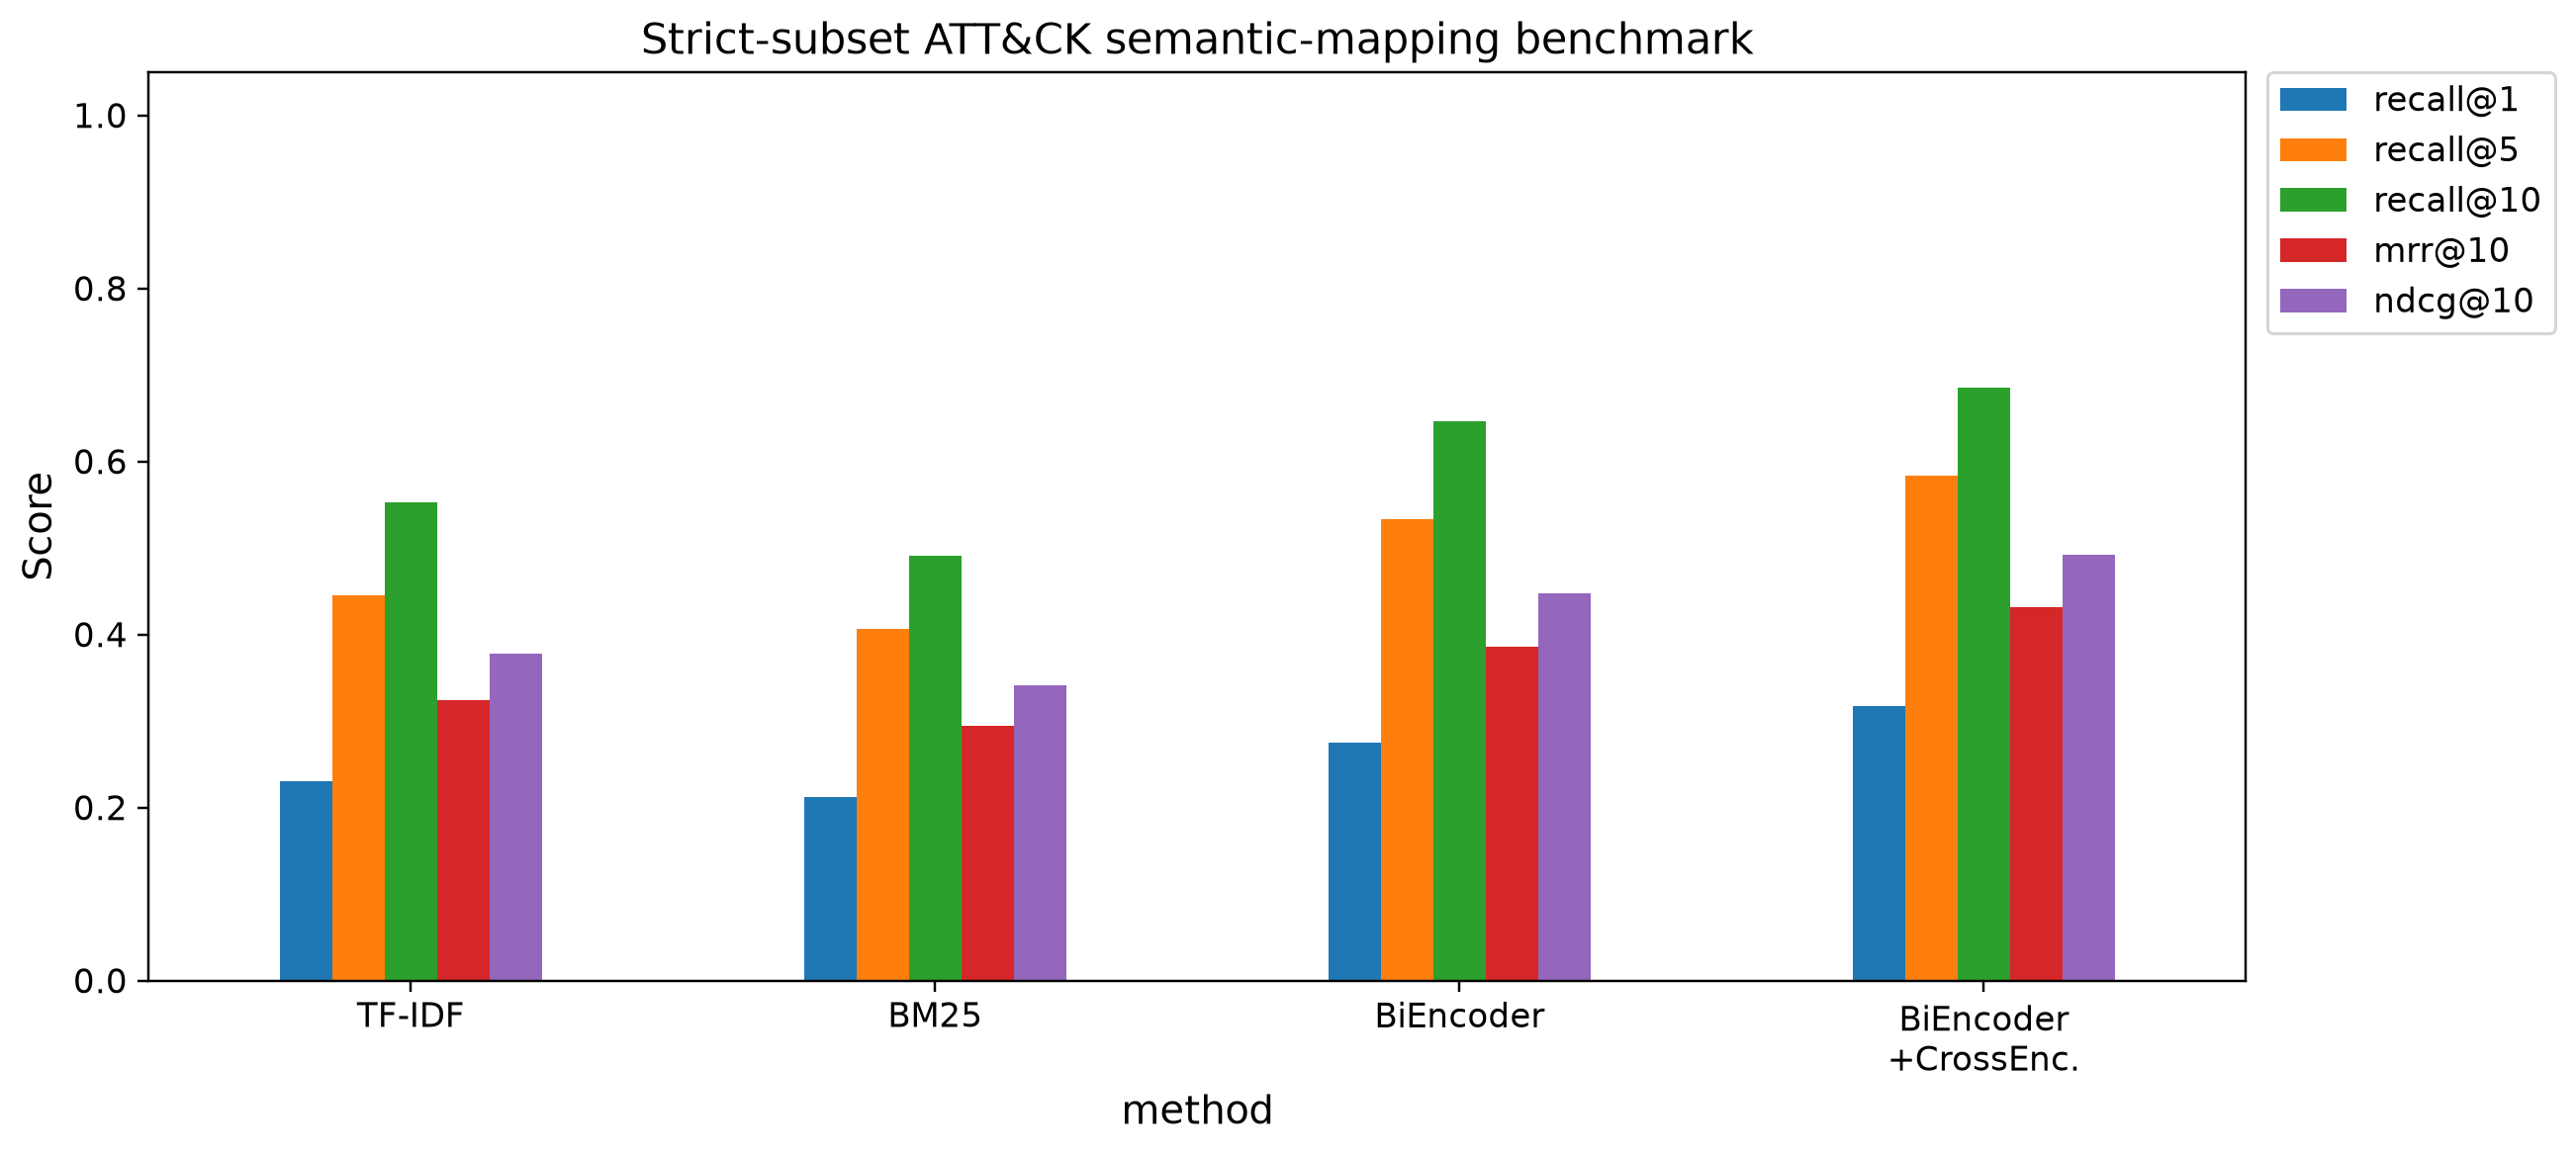
\includegraphics[width=\linewidth]{figures/04_strict_retrieval_benchmark.png}
\caption{Strict-subset retrieval benchmark across evaluated methods.}
\label{fig:strict-benchmark}
\end{figure}

\begin{figure}[htbp]
\centering
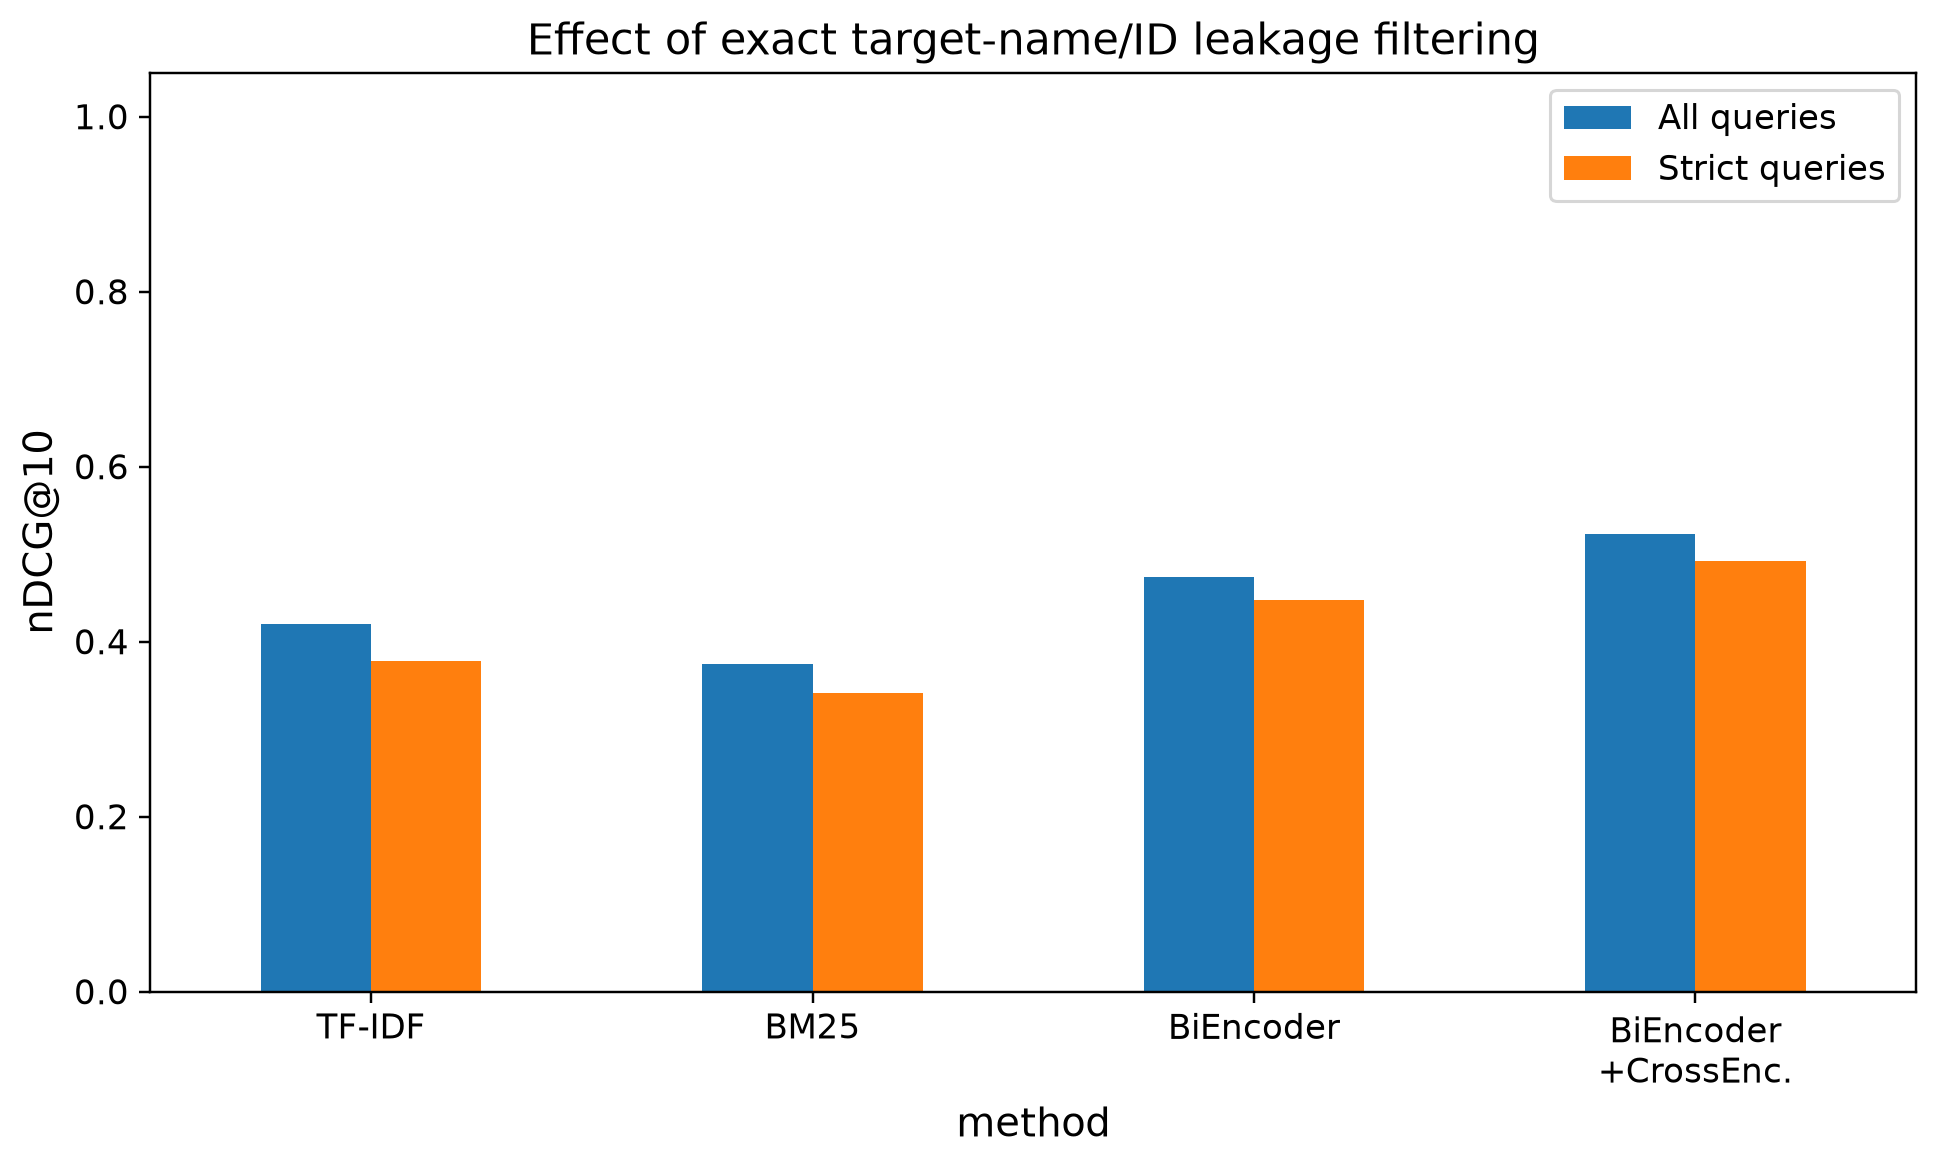
\includegraphics[width=\linewidth]{figures/05_all_vs_strict_ndcg.png}
\caption{nDCG@10 comparison between all-query and strict-query subsets.}
\label{fig:all-strict}
\end{figure}

\subsection{Cross-Encoder Reranking Gain}
Table~\ref{tab:reranking} isolates the strict-subset gain from cross-encoder reranking over the MiniLM bi-encoder. Reranking improved Recall@1 by 0.0418, MRR@10 by 0.0449, and nDCG@10 by 0.0437. Using the paired bootstrap of Section~\ref{sec:bootstrap}, the MRR@10 and nDCG@10 gains are statistically distinguishable from zero: +0.0449 MRR@10 [0.0389, 0.0510] and +0.0437 nDCG@10 [0.0385, 0.0491]. These gains indicate that joint query-candidate scoring improves the ordering of candidates already retrieved by the dense bi-encoder.

\begin{table}[htbp]
\caption{Strict-Subset Reranking Gain Over MiniLM Bi-Encoder}
\label{tab:reranking}
\centering
\begin{tabular}{lrrr}
\toprule
\textbf{Metric} & \textbf{Bi-enc.} & \textbf{Reranked} & \textbf{Gain} \\
\midrule
Recall@1 & 0.2750 & 0.3169 & 0.0418 \\
MRR@10 & 0.3862 & 0.4310 & 0.0449 \\
nDCG@10 & 0.4478 & 0.4915 & 0.0437 \\
\bottomrule
\end{tabular}
\vspace{2pt}
\begin{minipage}{0.95\linewidth}
\footnotesize Note: the Gain column is computed from full-precision (unrounded) per-query metric values, not from subtracting the two rounded columns shown here (e.g., $0.4310-0.3862=0.0448$ when subtracting the rounded values displayed, versus the reported full-precision gain of 0.0449).
\end{minipage}
\end{table}

\subsection{Computational Efficiency}
Table~\ref{tab:efficiency} reports computational efficiency. TF-IDF had the lowest mean query latency, while the bi-encoder provided stronger ranking quality with modest latency after candidate embeddings were available. Cross-encoder reranking increased mean latency to 228.03 ms/query because it scored 20 query-candidate pairs per query. Fig.~\ref{fig:latency} summarizes the quality-latency trade-off.

\begin{table}[htbp]
\caption{Efficiency Measurements From Full Execution}
\label{tab:efficiency}
\centering
\scriptsize
\begin{tabular}{p{2.6cm}rrrr}
\toprule
\textbf{Method} & \textbf{Index s} & \textbf{ms/q} & \textbf{Params} & \textbf{Mem.\ (MiB)}$^{*}$ \\
\midrule
TF-IDF & 0.119 & 0.016 & 0 & 0.0 \\
BM25 & 0.019 & 1.041 & 0 & 0.0 \\
MiniLM-BiEncoder & 6.892 & 1.354 & 22.7M & 86.6 \\
MiniLM-BiEncoder+ CrossEncoder & 6.892 & 228.030 & 45.4M & 173.3 \\
\bottomrule
\end{tabular}
\vspace{2pt}
\begin{minipage}{0.95\linewidth}
\footnotesize $^{*}$``Mem. (MiB)'' is the in-memory footprint of the model's learned parameters only (float32), not total process or runtime memory usage, which also includes activations, tokenizer/index structures, and framework overhead not measured here.
\end{minipage}
\end{table}

\begin{figure}[htbp]
\centering
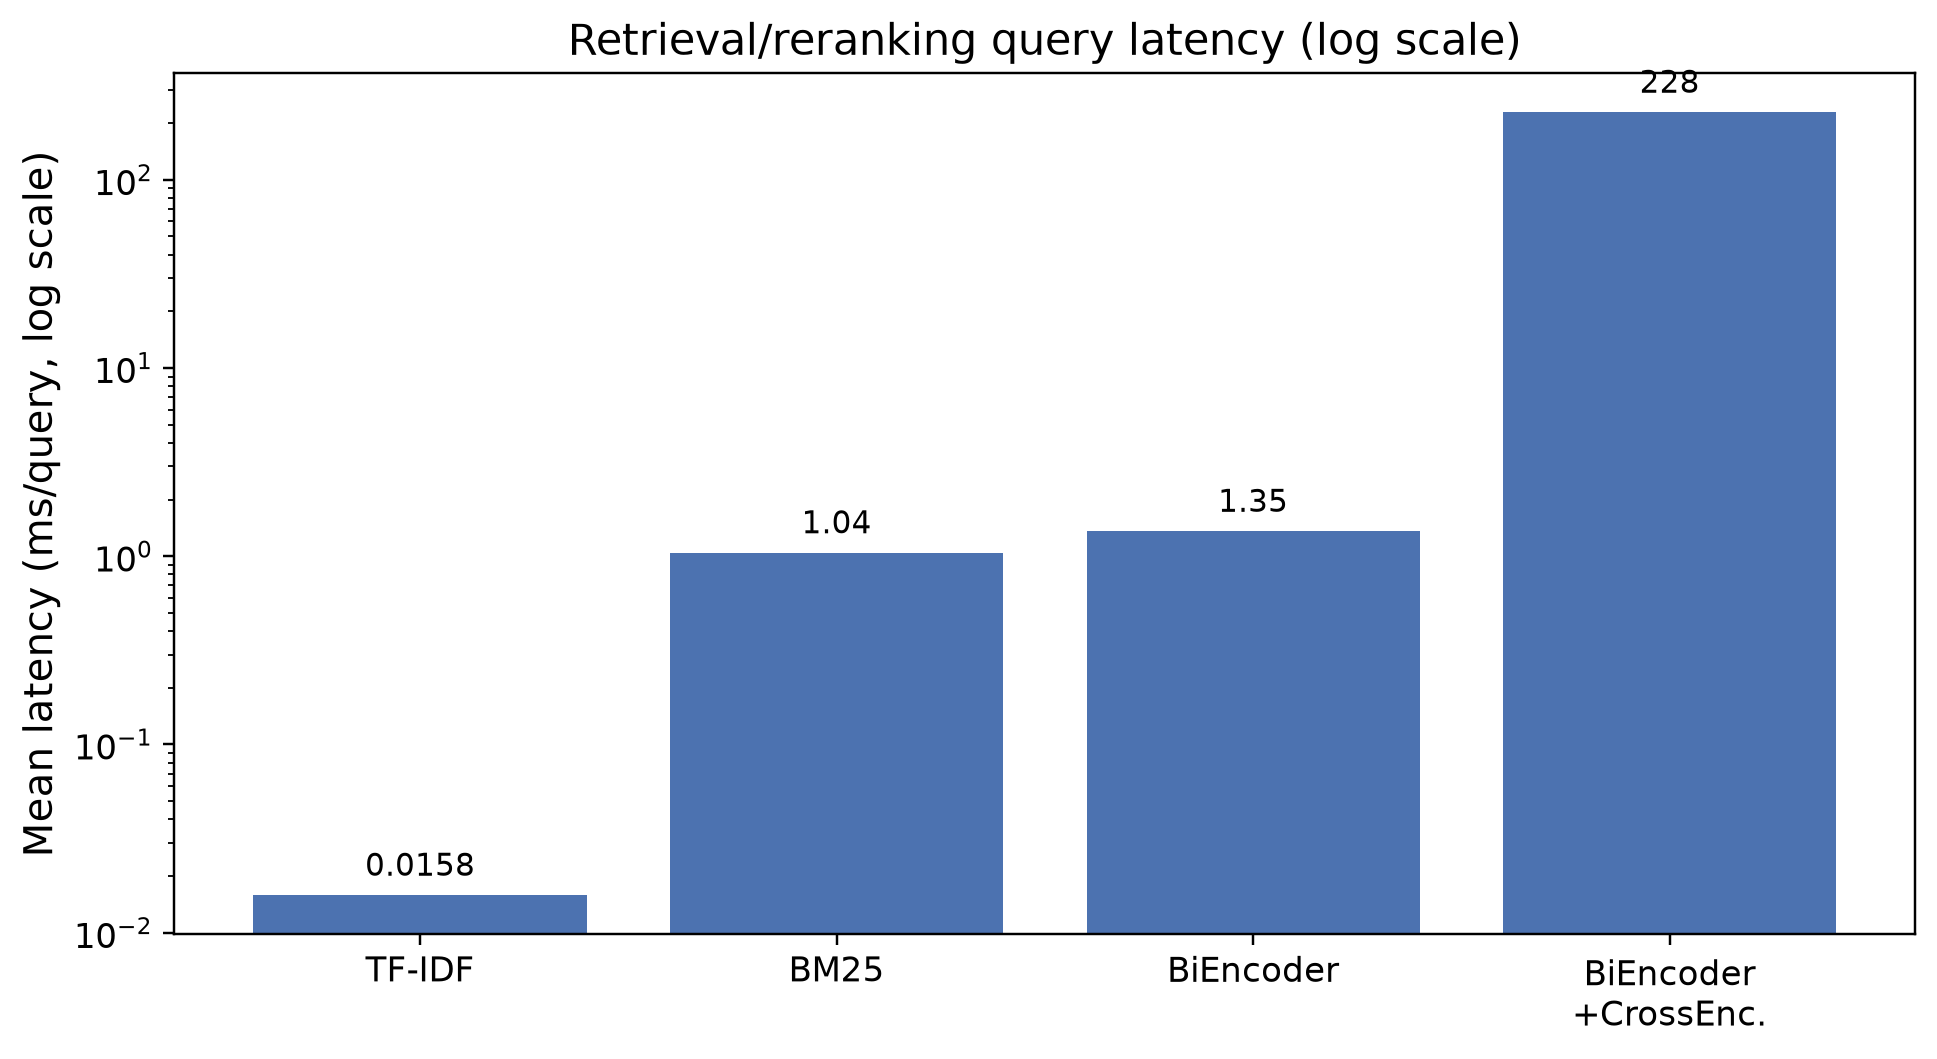
\includegraphics[width=\linewidth]{figures/06_query_latency.png}
\caption{Mean query latency for lexical, dense, and reranked retrieval, shown on a logarithmic axis with per-bar values annotated, since cross-encoder reranking latency is roughly two orders of magnitude larger than the other methods.}
\label{fig:latency}
\end{figure}

\subsection{Exploratory Attention and Error Analysis}
The full run generated an exploratory final-layer attention inspection for one correctly retrieved cross-encoder pair. The query concerned the 2015 Ukraine Electric Power Attack, and the top-ranked candidate was ATT\&CK T1570, Lateral Tool Transfer, marked relevant in the benchmark. The inspection is qualitative only; attention weights are not interpreted as causal explanations or feature importance. Fig.~\ref{fig:attention} presents the top token weights for this example.

\begin{figure}[htbp]
\centering
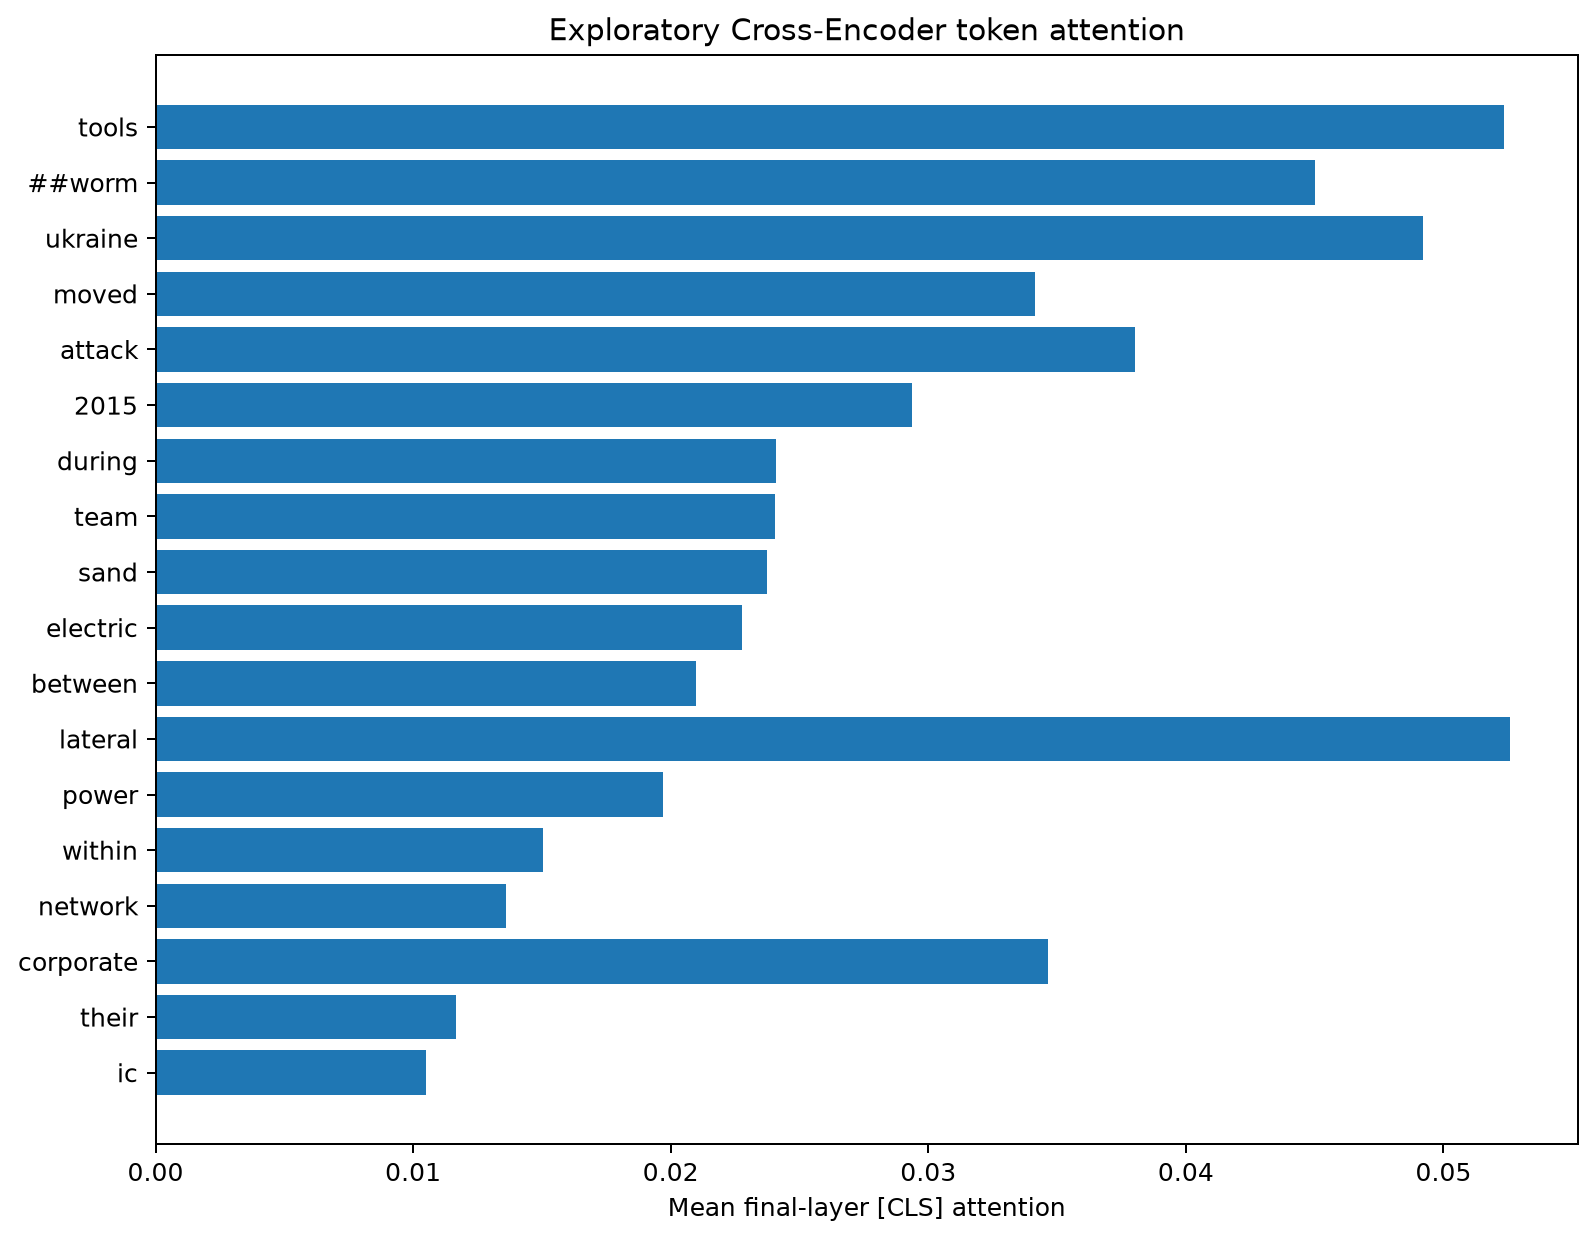
\includegraphics[width=0.88\linewidth]{figures/07_attention_top_tokens.png}
\caption{Exploratory token-weight visualization for one cross-encoder example. Attention is not treated as a causal explanation.}
\label{fig:attention}
\end{figure}

The strict cross-encoder output still contained 10,144 queries for which no relevant technique appeared at rank 1. This indicates that, although reranking improves aggregate metrics, the task remains difficult and cannot be reduced to a solved normalization problem.

To characterize these 10,144 strict rank-1 failures (saved in \url{results/strict_crossencoder_failure_cases.csv}), we checked, for each failing query, whether any relevant technique was present anywhere in the bi-encoder's top-20 candidates (the input to reranking). For 6,559 of 10,144 failures (64.7\%), a relevant technique \emph{was} present in the top-20 but the cross-encoder did not rank it first; for the remaining 3,585 (35.3\%), no relevant technique was present in the bi-encoder top-20 at all, so no reranking of that top-20 could have produced a correct rank-1 answer. This split indicates that a majority of remaining strict failures are reranking-ordering errors rather than initial-retrieval failures, but a substantial minority (over a third) reflect candidates that dense retrieval itself failed to surface.

Manual inspection of a sample of failures, without a formal inter-annotator taxonomy, suggests three recurring exploratory failure patterns, illustrated with unmodified examples from the failure-case file: (i) \emph{same-parent sub-technique confusion}, e.g., query Q000035 was top-ranked to T1059.001 (PowerShell) while the labeled relevant technique was the sibling sub-technique T1059.003 (Windows Command Shell), both under Command and Scripting Interpreter; (ii) \emph{parent-versus-sub-technique confusion}, e.g., query Q000045 was top-ranked to the parent technique T1036 (Masquerading) while the relevant label was its sub-technique T1036.004 (Masquerade Task or Service); and (iii) \emph{multi-relevant/insufficient-context queries}, where the query's short procedure text is compatible with several unrelated techniques, e.g., query Q000156 (``APT41 DUST used compromised Google Workspace accounts for command and control.'') was top-ranked to T1087.003 (Email Account) while the labeled relevant techniques were T1102 (Web Service) and T1586.003 (Cloud Accounts); 55 of the 91 multi-relevant queries were among the strict rank-1 failures. These categories are illustrative and exploratory rather than an exhaustive or independently validated taxonomy, since no manual multi-annotator labeling of the full failure set was performed.

\section{Discussion}
The results support three observations. First, dense semantic retrieval improved over the lexical baselines on both evaluation subsets. On the strict subset, MiniLM bi-encoder nDCG@10 exceeded TF-IDF by 0.0703 and BM25 by 0.1067. This suggests that pretrained sentence embeddings capture useful semantic correspondences between procedure descriptions and ATT\&CK technique descriptions beyond exact target-name overlap.

Second, cross-encoder reranking improved the ordering of the bi-encoder candidate set. The strict nDCG@10 gain of 0.0437 and MRR@10 gain of 0.0449 are meaningful in the context of a 697-candidate ranking task. Because reranking was limited to the top-20 dense candidates, these gains reflect improved local ordering rather than full-corpus retrieval.

Third, ranking quality must be considered jointly with computational cost. The cross-encoder achieved the best effectiveness metrics but was roughly two orders of magnitude slower per query than the bi-encoder in this CPU execution. For interactive analyst workflows, this may be acceptable when applied to short candidate lists. For high-throughput pipelines, the bi-encoder may offer a more practical balance.

\section{Limitations}
\label{sec:limitations}
The benchmark uses candidate documents and procedure queries derived from the same ATT\&CK knowledge base. It therefore evaluates ATT\&CK-derived semantic mapping, not generalization to independent external CTI reports. The strict subset removes exact target identifiers and exact target technique names, but it does not eliminate all possible lexical overlap. The evaluated Transformer models were pretrained and used zero-shot; no ATT\&CK-specific supervised fine-tuning was performed. Public pretrained models may have seen cybersecurity text during pretraining. Cross-encoder reranking is constrained by the bi-encoder top-20 candidates and cannot recover relevant techniques outside that set. Attention visualizations are included only as exploratory diagnostics, not as causal explanations. The bootstrap confidence intervals reported in Section~\ref{sec:results} resample at the query level (Section~\ref{sec:bootstrap}); because procedure queries are grouped from STIX \texttt{uses} relationships and multiple queries can derive from the same underlying source object (e.g., the same threat group or software), queries are not fully independent, and this dependence structure is not modeled by query-level resampling, so the reported confidence intervals may understate the true sampling uncertainty. Finally, the accompanying Streamlit interface is a research demonstrator and does not implement SIEM integration, SOC workflow automation, retrieval-augmented generation, or automated incident response.

\section{Conclusion}
This paper presented a reproducible retrieval and reranking benchmark for mapping ATT\&CK-derived CTI procedure descriptions to Enterprise ATT\&CK techniques and sub-techniques. In the full execution, the benchmark included 697 candidate techniques and 17,030 procedure queries, with 14,868 queries retained after exact target-name and target-ID leakage auditing. Pretrained MiniLM bi-encoder retrieval improved over TF-IDF and BM25, and cross-encoder reranking produced the strongest top-10 ranking metrics under both all-query and strict-query evaluation. These findings indicate that Transformer-based semantic retrieval is useful for ATT\&CK mapping under the evaluated conditions, while the remaining error cases and latency costs show that analyst-facing deployment should preserve human review and transparent candidate ranking.

\section*{Data Availability}
The benchmark is constructed from the official MITRE ATT\&CK Enterprise STIX 2.1 data, obtained from the canonical MITRE repository \cite{mitre_attack_stix_data}; this study does not redistribute the raw third-party STIX bundle. The full execution manifest (\texttt{results/experiment\_manifest.json}) records the source URL, the SHA-256 hash of the exact bundle used, the STIX object count, candidate-technique count, all/strict query counts, the strict-subset rule, model identifiers, software versions, and the completion timestamp, so that the exact benchmark instance can be independently verified. Reproducibility metadata and derived artifacts (metrics, per-query metrics, rankings, efficiency measurements, model metadata, and bootstrap confidence intervals) are made available through the research repository referenced under Code Availability.

\section*{Code Availability}
The source code, experimental configurations, reproducibility scripts, and supporting artifacts associated with this study are available at:

\url{https://github.com/PesquisaDoug/mitre-attack-semantic-mapping-benchmark}

\section*{Article Archive}
This manuscript and its associated research archive are deposited on Zenodo.

\noindent Zenodo DOI: \verb|10.5281/zenodo.22821273|

\noindent \url{https://doi.org/10.5281/zenodo.22821273}

\bibliographystyle{IEEEtran}
\bibliography{references}

\end{document}
